\documentclass{beamer}
\usetheme{Madrid}
\usepackage[T2A]{fontenc}
\usepackage[utf8]{inputenc}
\usepackage[english,russian]{babel}
\usepackage{graphicx}
\usepackage{xcolor}
\usepackage{amsmath}
\usepackage{mathtools}
\usepackage{bm}
\usepackage{bbm}
\usepackage{pifont}
\usepackage{physics}
\usepackage{hyperref}
\usepackage{appendixnumberbeamer}
\usepackage[backend=biber]{biblatex}
\addbibresource{rudakov-etapipi-2025.bib}

\makeatletter
\renewrobustcmd{\blx@mkbibfootnote}[2]{%
  \iftoggle{blx@footnote}
    {\blx@warning{Nested notes}%
     \addspace\mkbibparens{#2}}
    {\unspace
     \ifnum\blx@notetype=\tw@
       \expandafter\@firstoftwo
     \else
       \expandafter\@secondoftwo
     \fi
       {\csuse{blx@theendnote#1}{\protecting{\blxmkbibnote{end}{#2}}}}
       {\csuse{footnote}[frame]{\protecting{\blxmkbibnote{foot}{#2}}}}}}
\makeatother

\title[$e^+e^-\rightarrow\eta\pi^+\pi^-$]{Изучение процесса $e^+e^-\to\eta\pi^+\pi^-$ с детектором КМД-3}
\author{Грибанов Сергей Сергеевич}
\date{\today}


\begin{document}

\frame{\titlepage}

\begin{frame}
  \frametitle{Мотивация}
  \begin{itemize}
  \item Изучение динамики.
  \item Вычисление $\mathcal{B}()$, тест CVC-гипотезы.
  \item Получение форм-фактора $\eta\to\gamma^{\star}\gamma^{\star}$.
  \item Вклад в $(g-2)_{\mu}$.
  \end{itemize}
\end{frame}

\begin{frame}
  \frametitle{Коллайдер ВЭПП-2000}
  \begin{minipage}[t]{0.49\linewidth}
    \begin{figure}
      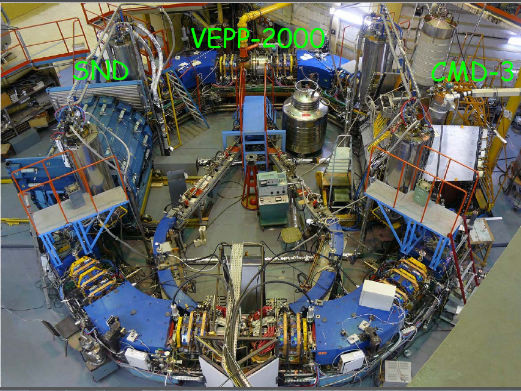
\includegraphics[width=\linewidth]{figures/vepp2k.png}
    \end{figure}
  \end{minipage}
  \begin{minipage}[t]{0.5\linewidth}
    \scriptsize
    \begin{itemize}
    \item Область сканирования $A < \sqrt{s} < B$.
    \item Энергия измеряется методом обратного комптоновского рассеяния с точностью
      $50\text{ КэВ}$.
    \item Выпервые использована методика круглых пучков.
    \item Достигнута светимость
      $6\times{10^{31}}\text{ см}^{-2}\text{с}^{-1}$~(проектная~$\sim{10^{32}}\text{ см}^{-2}\text{c}^{-1}$).
    \item Два детектора КМД-3 и СНД.
    \end{itemize}
  \end{minipage}
\end{frame}

\begin{frame}
  \frametitle{Детектор КМД-3}
  \begin{minipage}[t]{0.4\linewidth}
    \begin{figure}
      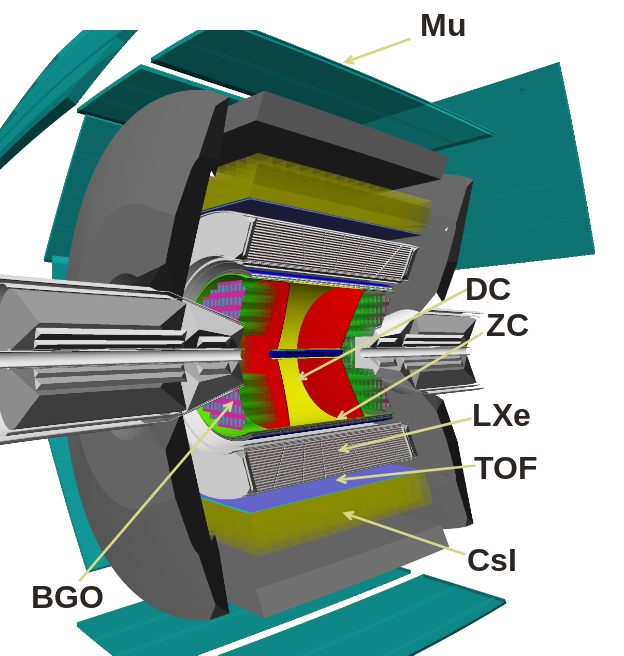
\includegraphics[width=\linewidth]{figures/cmd3.png}
    \end{figure}
  \end{minipage}
  \begin{minipage}[t]{0.55\linewidth}
    \scriptsize
    \begin{itemize}
    \item ДК: $1218$ гексоганальных ячеек с сигнальными и полевыми проволочками
      (W-Re слав, диаметр $15\text{ мкм}$); пространственное разрешение
      $\sigma_{R\phi}\sim{100}\text{ мкм}$, $\sigma_{Z}\sim{2.5}\text{ мм}$, $\sigma{P}/P\sim{?}$.
    \item Сверхпроводящий соленоид с магнитным полем~$\sim{1.3}\text{ Тл}$.
    \item Z-камера
    \item LXe калориметр: ширина $5.1\text{ }X_0$, 196 башен и 1286 полосок,
      пространственное разрешение $1$-$2\text{ мм}$, энергетическое~(для
      конверсии фотонов) $\sigma{E}/E\sim 0.034/\sqrt{E}\text{[ГэВ]}\oplus{0.020}$.
    \item CsI калориметр: ширина $8\text{ }X_0$, 1152 кристалла.
    \item TOF:
    \item Mu:
    \end{itemize}
  \end{minipage}
\end{frame}

\begin{frame}
  \frametitle{Критерии отбора событий}
  \scriptsize
  \begin{itemize}
    \item Наличие двух центральных треков
    \item Наличие двух или более фотонов с энергиями больше $50\text{ МэВ}$.
    \item Суммарное энерговыделение кандидатов на $\pi^+$ и $\pi^-$ в калориметре меньше
      $0.4 + 0.25\times(\sqrt{s} - 1.2)$~ГэВ для подавления событий $e^+e^-$ рассеяния.
    % \item В зависимостях $\dv{E(p)}{x}$ для кандидатов в $\pi^{\pm}$ вырезается (мягко) области
    %   отвечающие $\pi$-мезонам.
    \item Кинематическая реконструкция\footfullcite{Gribanov_2023}
      в гипотезе $e^+e^-\rightarrow\pi^+\pi^-\gamma\gamma$: фит должен сойтись
      и $\chi^2<40$.
    \item Кинематическая реконструкция в гипотезе $e^+e^-\rightarrow\pi^+\pi^-\gamma\gamma\gamma\gamma_{\text{lost}}$. Одна
      пара фотонов складывается в $\pi^0$ (для которой $\chi^2$ меньше). Требуется, чтобы
      либо фит не сошелся, либо фит сошелся и $\chi^2>20$.
    \item Кинематическая реконструкция в гипотезе $e^+e^-\rightarrow\eta\pi^+\pi^-$, $\eta\rightarrow\gamma\gamma$. Требуется,
      чтобы фит сошелся, но никаких ограничений на $\chi^2$ не накладывается. Нужна
      для того, чтобы в амплитудном фите четырех-импульс двух фотонов
      соответствовал четырех-импульсу $\eta$-мезона.
  \end{itemize}
\end{frame}

\begin{frame}
  \frametitle{Оперделение числа сигнальных событий}
\end{frame}

\begin{frame}
  \frametitle{Амплитудный анализ процесса $e^+e^-\to\eta\pi^+\pi^-$}
  \begin{minipage}[t]{0.49\linewidth}
  \scriptsize
  \textbf{Промежуточные состояния}\\
  \textit{Достоверно наблюдаются:}
  \begin{itemize}
  \item {\scriptsize $\rho(770)\eta$ --- P-волна.} 
  \item {\scriptsize $a_2(1320)\pi$ --- D-волна.}
  \end{itemize}
  \textit{Изучались, но дают малый вклад:}
  \begin{itemize}
  \item {\scriptsize $\omega\pi$~($\rho$-$\omega$ смешивание) --- P-волна.}
  \item {\scriptsize $\rho(1450)\pi$ --- P-волна.}
  \item {\scriptsize $\rho(1700)\pi$ --- P-волна.}
  \item {\scriptsize $a_2(1700)\pi$ --- D-волна.}
  \end{itemize}
  \vspace{1em}%
  \textbf{Плотность вероятности}
  \vspace{-1em}%
   \begin{eqnarray*}
     \begin{split}
     \textstyle
       &f(\Phi; \bm{C}_{\text{sig}}, \bm{C}_{\text{bkg}}) =
     \frac{1}{N_{\text{tot}}(\bm{C}_{\text{sig}}, \bm{C}_{\text{bkg}})}\times\\
       &\left[ \varepsilon_{\text{phsp
    sig}}(\Phi)\text{I}_{\text{sig}}(\Phi; \bm{C}_{\text{sig}}) + \text{I}_{\text{bkg}}(\Phi;
         \bm{C}_{\text{bkg}}) \right],
     \end{split}
   \end{eqnarray*}
   где $\textstyle\bm{C}_{\text{sig}}$ --- параметры модели сигнального процесса,
   $\textstyle\bm{C}_{\text{bkg}}$ --- параметры модели фонового процесса;
   $\textstyle\varepsilon_{\text{phsp sig}}$ --- эффективность событий сигнала, разыграных по
   фазовому объему; $\textstyle{}\text{I}_{\text{bkg}}$ --- функция, описывающая распреде-
\end{minipage}
\begin{minipage}[t]{0.49\linewidth}
  \scriptsize
  ление~(зарегестрированных) событий фонового процесса в переменных сигнального
  процесса; $\textstyle{}\text{I}_{\text{sig}}$ --- усредненный по поляризациям начальных частиц
  квадрат модуля суммарной амплитуды сигнального процесса; $\textstyle{}N_{\text{tot}}$ ---
  нормировка: $\textstyle{}N_{\text{tot}} = N_{\text{sig}} + N_{\text{bkg}}$,
  $\textstyle{}N_{\text{sig}}=\int\varepsilon_{\text{sig}}(\Phi)\text{I}_{\text{sig}}(\Phi;\bm{C}_{\text{sig}})\dd{\Phi}$,
  $\textstyle{}N_{\text{bkg}}=\int{}\text{I}_{\text{bkg}}(\Phi; \bm{C}_{\text{bkg}})\dd{\Phi}$.\\
  Функцию $\text{I}_{\text{sig}}$
  можно записать в виде\footnote{\scriptsize Массы и ширины резонансов полагаются
    фиксированными.}:
  $\textstyle{}\text{I}_{\text{sig}}=\bm{C}^{\dag}_{\text{sig}}\hat{\rho}_{\text{sig}}(\Phi)\bm{C}_{\text{sig}}$,
  где $\textstyle{}\hat{\rho}^{\dag}_{\text{sig}}=\hat{\rho}_{\text{sig}}$,
  $\textstyle{}\bm{C}_{\text{sig}}\in\mathbb{C}^{n_{\text{sig}}}$.
  Тогда $\textstyle{}N_{\text{sig}}=\bm{C}^{\dag}_{\text{sig}}\hat{\text{I}}_{\text{sig}}\bm{C}_{\text{sig}}$,
  где
  $\textstyle{}\hat{\text{I}}_{\text{sig}}=\frac{1}{N^{\text{MC}}_{\text{phsp sig}}}\sum_{j\in\text{phsp sig}}\hat{\rho}_{\text{sig}}(\Phi_j)$.\\
  Функцию $\textstyle{}\text{I}_{\text{bkg}}$ можно записать в виде:
  $\textstyle{}\text{I}_{\text{bkg}}=\bm{C}^{\dag}_{\text{bkg}}\hat{\rho}_{\text{bkg}}\bm{C}_{\text{bkg}}$, где
  $\textstyle{}\hat{\rho}^{\dag}_{\text{bkg}}=\hat{\rho}_{\text{bkg}}$, $\hat{\rho}_{\text{bkg}}$ ---
  дигональная матрица, $\bm{C}_{\text{bkg}}\in\mathbb{R}^{n_{\text{bkg}}}$. Тогда
  $\textstyle{}N_{\text{bkg}}=\bm{C}^{\dag}_{\text{bkg}}\hat{\text{I}}_{\text{bkg}}\bm{C}_{\text{bkg}}$, где
  $\textstyle{}\hat{\text{I}}_{\text{bkg}}=\frac{1}{N^{\text{MC}}_{\text{phsp sig}}}\sum_{j \in \text{phsp sig}}\frac{\hat{\rho}_{\text{bkg}}(\Phi_j)}{\varepsilon_{\text{phsp sig}}(\Phi_j)}$.
\end{minipage}
\end{frame}

\begin{frame}
  \frametitle{Extended~Maximum~Likelihood~(EML)\footfullcite{BARLOW1990496}}
  \scriptsize
  \begin{eqnarray*}
    \textstyle
    \begin{split}
      &\mathcal{L}_{\text{ext}} = \frac{N^{N_{\text{exp}}}_{\text{tot}}}{N_{\text{exp}}!}e^{-N_{\text{tot}}}\prod_{\ell \in \text{exp.}}f(\Phi_{\ell};\bm{C}_{\text{sig}},\bm{C}_{\text{bkg}}) = \frac{1}{N_{\text{exp}}!}e^{-N_{\text{tot}}}\prod_{\ell \in \text{exp.}}N_{\text{tot}}f(\Phi_{\ell};\bm{C}_{\text{sig}},\bm{C}_{\text{bkg}}) \\
      &\boxed{%
       \ln{\mathcal{L}_{\text{ext}}} = \sum_{\ell \in \text{exp}}\ln{\left(
        {\bm{C}^{\dag}}_{\text{sig}}\hat{\rho}_{\text{sig}}(\Phi_{\ell})\bm{C}_{\text{sig}} +
        \bm{C}^{\dag}_{\text{bkg}}\frac{\hat{\rho}_{\text{bkg}}(\Phi_{\ell})}{\varepsilon_{\text{phsp sig}}(\Phi_{\ell})}\bm{C}_{\text{bkg}} \right)} - {\bm{C}^{\dag}}_{\text{sig}}\hat{\text{I}}_{\text{sig}}\bm{C}_{\text{sig}} - {\bm{C}^{\dag}}_{\text{bkg}}\hat{\text{I}}_{\text{bkg}}\bm{C}_{\text{bkg}}%
        }
    \end{split}
  \end{eqnarray*}
  \begin{itemize}
    \item Позволяет найти полное число событий~($N_{\text{tot}}=N_{\text{sig}} + N_{\text{bkg}}$) при фите, число
      событий
      сигнала~($N_{\text{sig}}={\bm{C}^{\dag}}_{\text{sig}}\hat{\text{I}}_{\text{sig}}\bm{C}_{\text{sig}}$)
      и
      фона~($N_{\text{bkg}}={\bm{C}^{\dag}}_{\text{bkg}}\hat{\text{I}}_{\text{bkg}}\bm{C}_{\text{bkg}}$).
      Эти числа событий согласуются с аналогичными числами, полученными при фите
      спектра масс двух фотонов.
    \item Матрицы $\hat{\rho}_{\text{sig}}(\Phi_{\ell})$,
      $\frac{\hat{\rho}_{\text{bkg}}(\Phi_{\ell})}{\varepsilon_{\text{sig}}(\Phi_{\ell})}$,
      $\hat{\text{I}}_{\text{sig}}$ и $\hat{\text{I}}_{\text{bkg}}$ рассчитываются
      перед фитом.
    \item В данном анализе $\hat{\rho}_{\text{bkg}}(\Phi_{\ell})$ --- матрица $1\times{1}$, т.к.
      рассматривается фон только от $e^+e^-\rightarrow\pi^+\pi^-\pi^0\pi^0$~(по фазовому объему).
    \end{itemize}
  \end{frame}

  \begin{frame}
  \frametitle{Метод нахождения $\varepsilon_{\text{phsp sig}}(\Phi)$ и $\hat{\rho}_{\text{bkg}}(\Phi)$}
  \scriptsize
  Эффективность сигнала $\varepsilon_{\text{phsp sig}}(\Phi)$ и плотность вероятности фона
  $\hat{\rho}_{\text{bkg}}(\Phi)$ в переменных трех-частичного процесса находились с
  помощью Kernel Density Estimation (KDE) с некоторыми
  модификациями\footfullcite{Poluektov_2015}. Для трех-частичных процессов можно
  указать $5$ независимых кинематических переменных. Были выбраны следующие
  переменные:
  \begin{itemize}
  \item $m^2_{\pi^+\pi^-}$,
  \item $m^2_{\eta\pi^-}$,
  \item $\cos\theta_{\eta}$,
  \item $\phi_{\eta}$,
  \item угол между плоскостями ($\vec{p}_{\pi^+}$, $\vec{p}_{\pi^-}$) и ($\vec{p}_{\eta}$, $\vec{e}_z$).
  \end{itemize}
  Так как пучки неполяризованные, то от угла $\phi_{\eta}$ ничего не зависит~(в
  пренебрежении неработающими каналами и т.п.).
\end{frame}


\begin{frame}
  \frametitle{Эффективность сигнала, $\varepsilon_{\text{phsp sig}}$}
    \begin{center}
    \begin{minipage}[t]{0.4\linewidth}
      \begin{figure}
        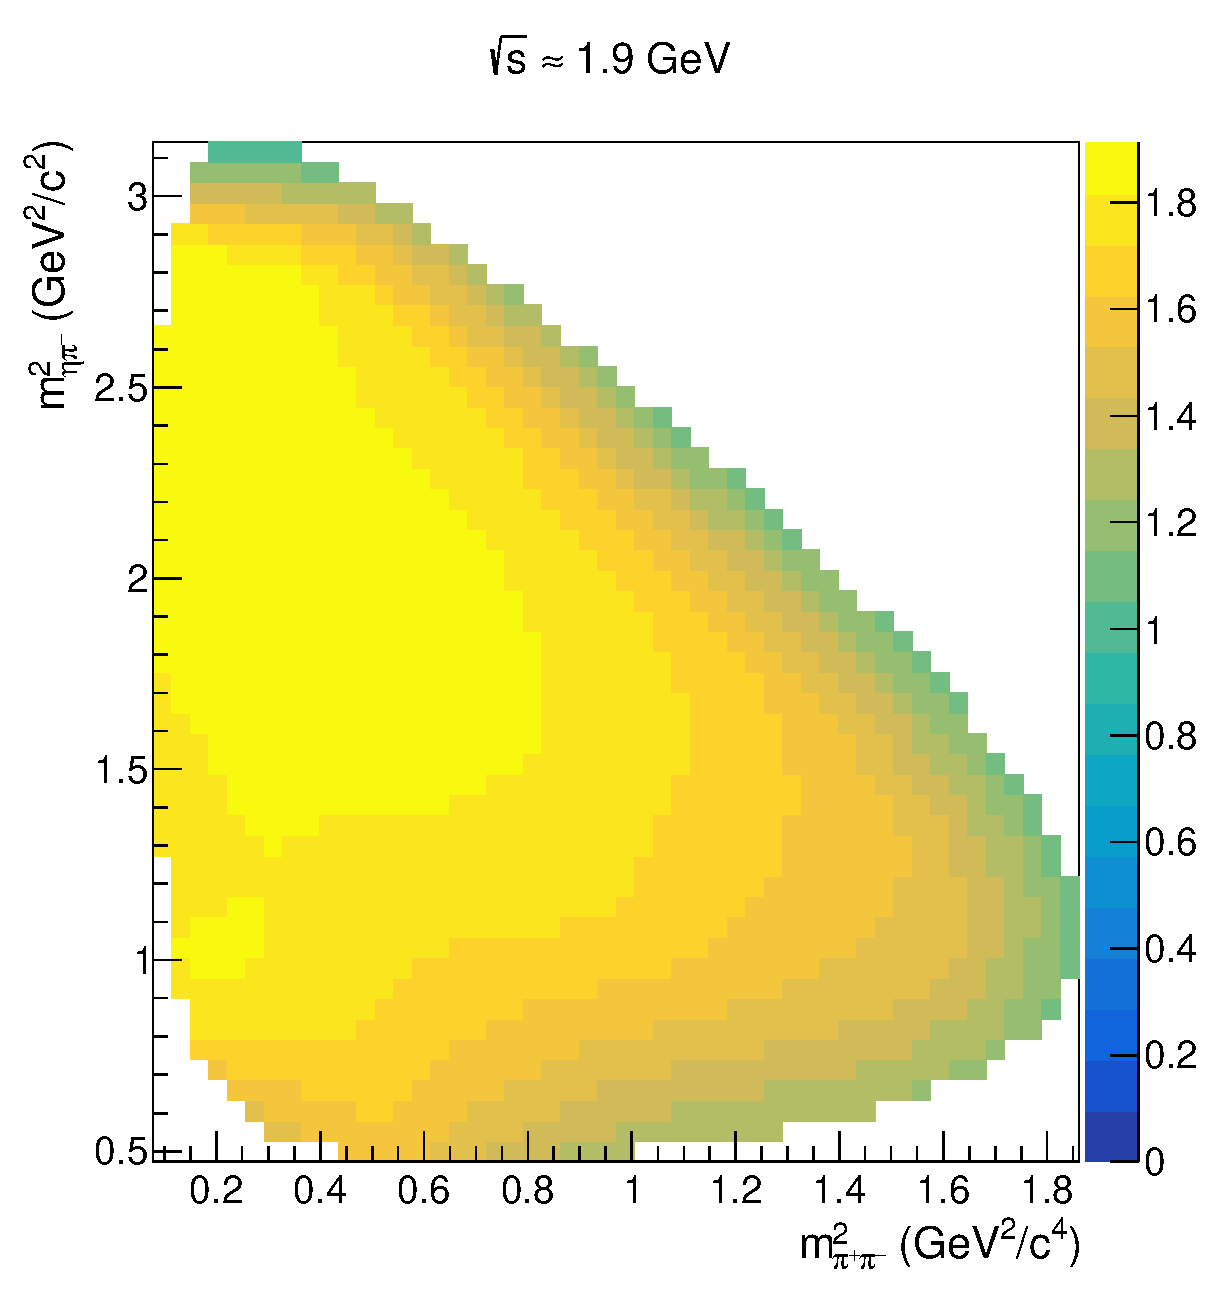
\includegraphics[width=\linewidth]{figures/kde_xy_signal.eps}
      \end{figure}
    \end{minipage}
    \begin{minipage}[t]{0.4\linewidth}
      \begin{figure}
        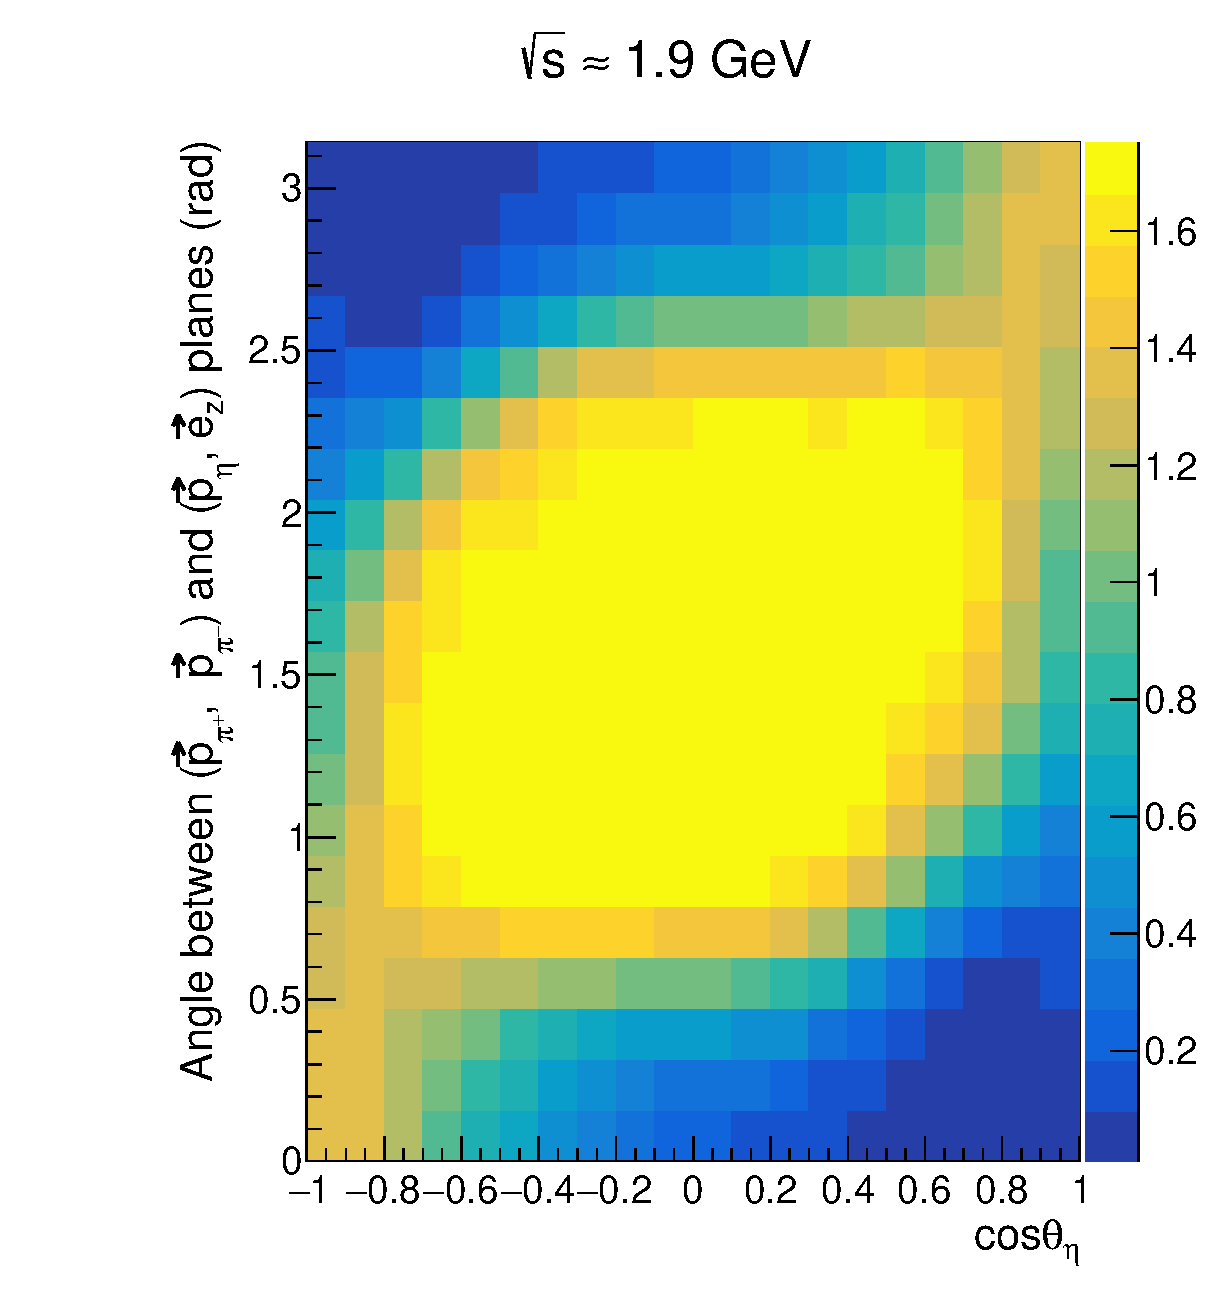
\includegraphics[width=\linewidth]{figures/kde_zu_signal.eps}
      \end{figure}
    \end{minipage}
  \end{center}
  \scriptsize
  Эффективность моделирования сигнала по фазовому объему в срезе по некоторым переменным (не интеграл, а значения
  PDF). В данной группе точек (вблизи $\sqrt{s}\approx 1.9\text{ GeV}$) оценка $\varepsilon_{\text{sig}}$ проведена с
  использованием~$\approx{}7.9\times{}10^6$ событий моделирования сигнала по фазовому
  объему~(после наложения всех критериев отбора).
\end{frame}

\begin{frame}
  \frametitle{Распределение фона, $\hat{\rho}_{\text{bkg}}$}
  \begin{center}
    \begin{minipage}[t]{0.4\linewidth}
      \begin{figure}
        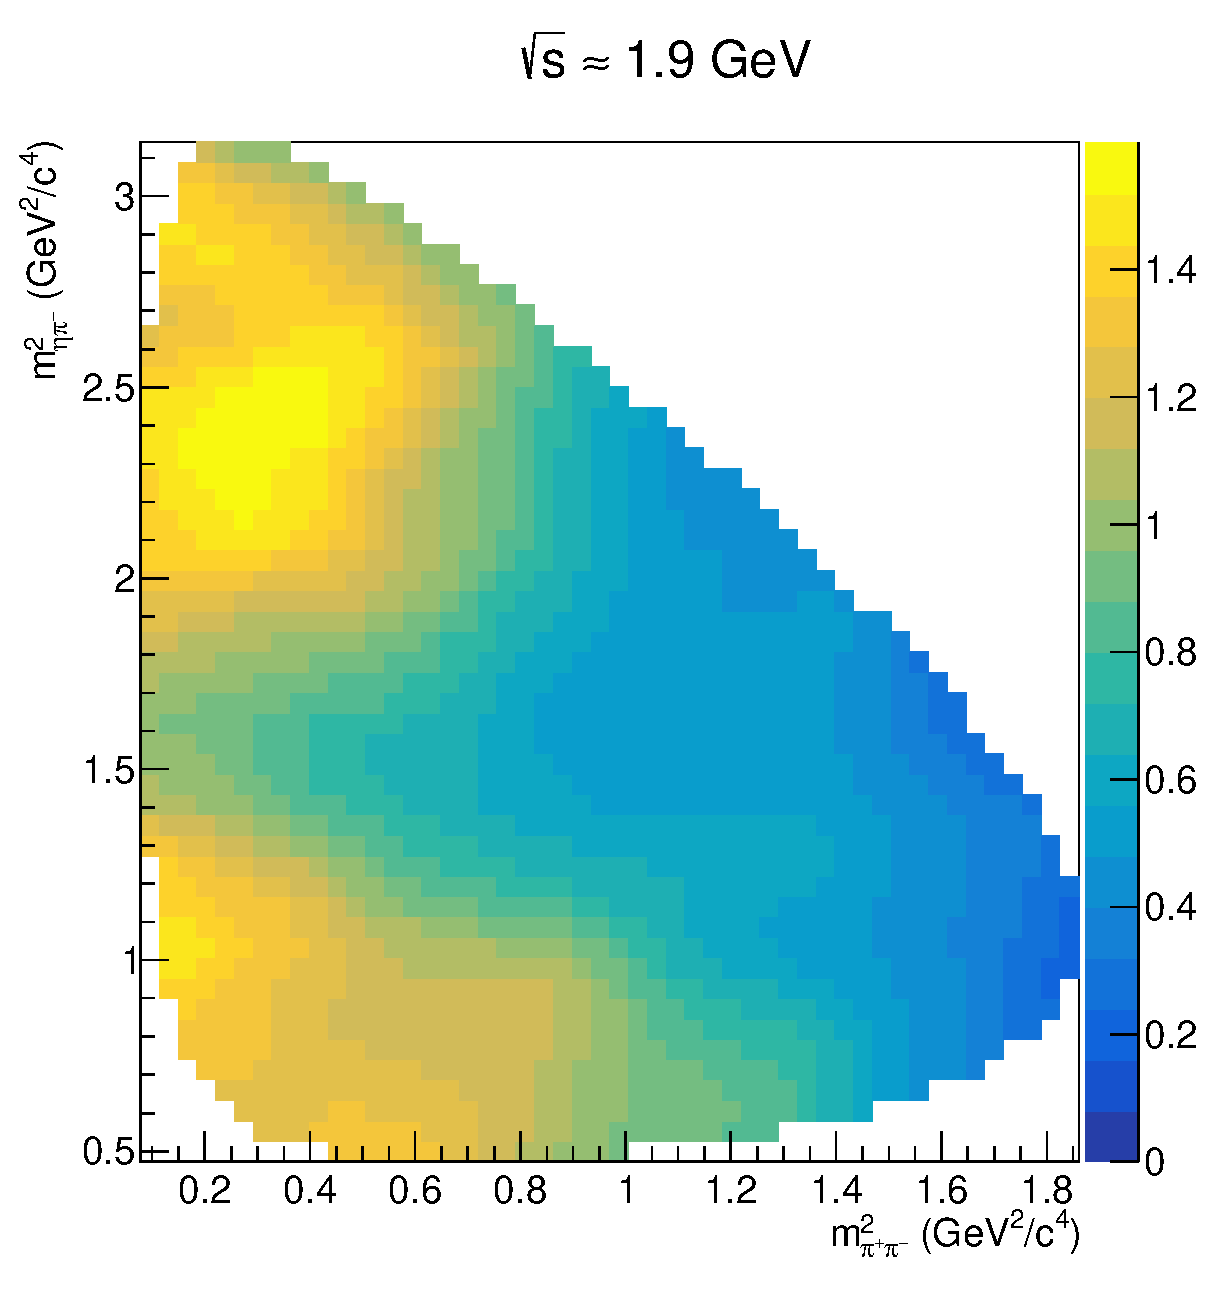
\includegraphics[width=\linewidth]{figures/kde_xy_background.eps}
      \end{figure}
    \end{minipage}
    \begin{minipage}[t]{0.4\linewidth}
      \begin{figure}
        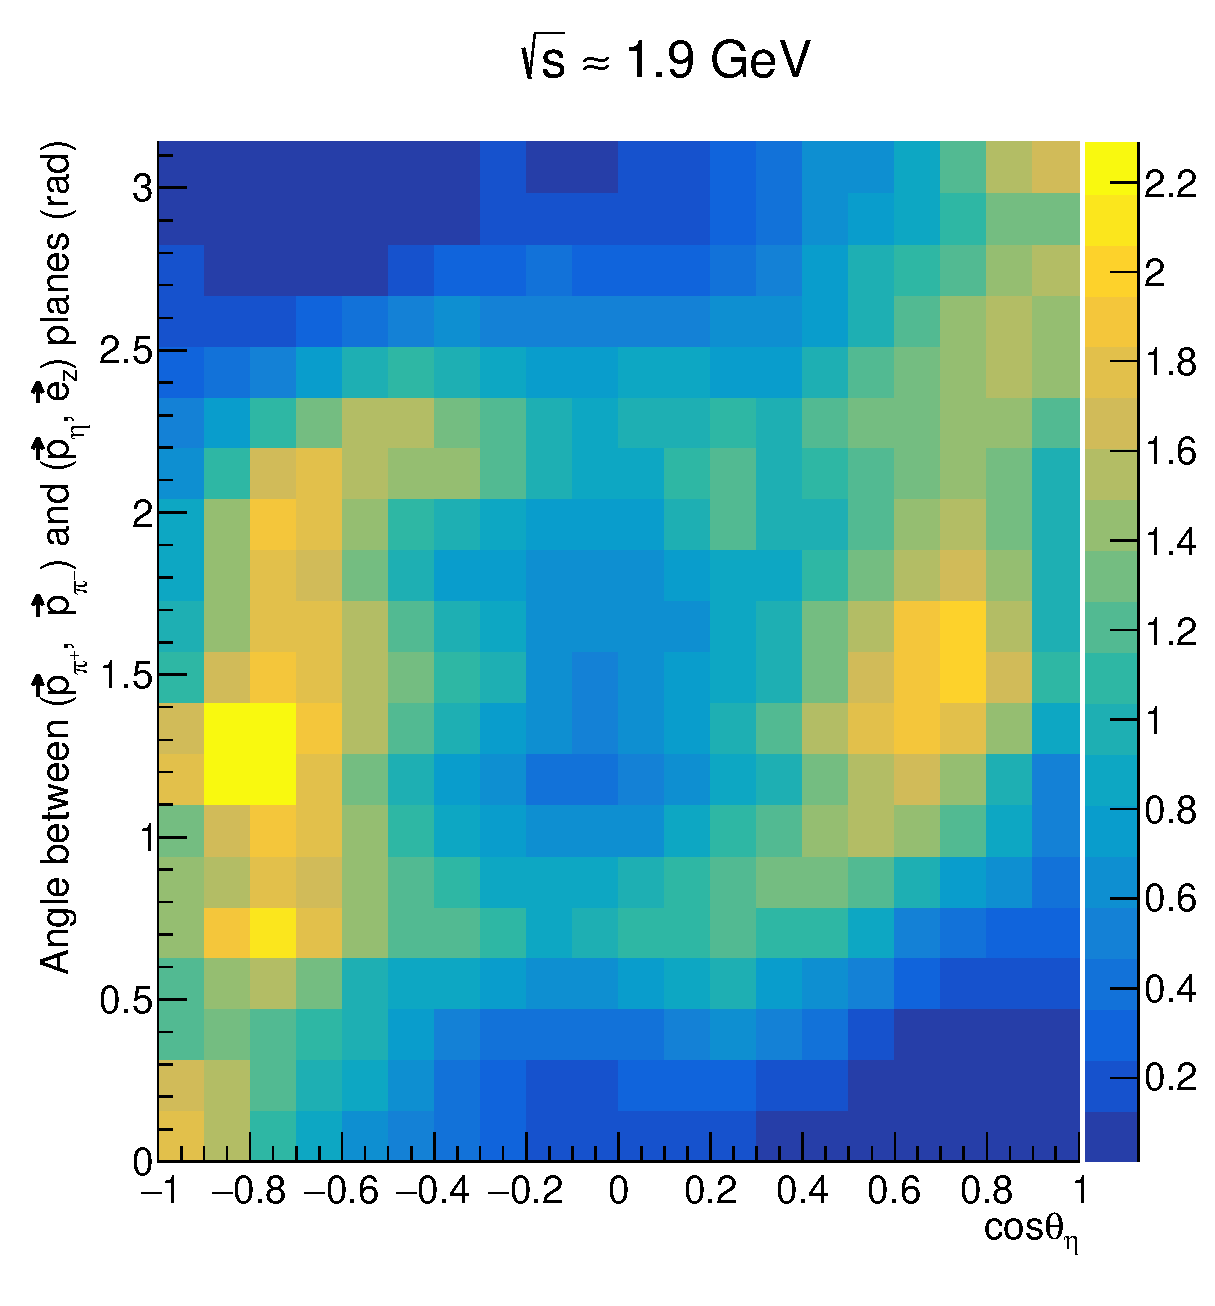
\includegraphics[width=\linewidth]{figures/kde_zu_background.eps}
      \end{figure}
    \end{minipage}
  \end{center}
  \scriptsize
  Плотность вероятности фона ($e^+e^-\rightarrow\pi^+\pi^-\pi^0\pi^0$ по фазовому объему) в срезе по
  некоторым переменным.  данной группе точек (вблизи $\sqrt{s}\approx 1.9\text{ GeV}$)
  оценка плотности фона была проведена по 15017 событиям (в других
  энергетических группах и того меньше). Далее будет показано, что это как-то
  работает~(т.к. фон меняется плавно, $\sigma$ для KDE выбран большим).
  \textbf{Актуализировать числа!!!!!!}
\end{frame}


\begin{frame}
  \frametitle{Сравнение спектров, $\sqrt{s}\approx{1.9}\text{ ГэВ}$}
  \begin{minipage}[t]{0.48\linewidth}
    \begin{figure}
      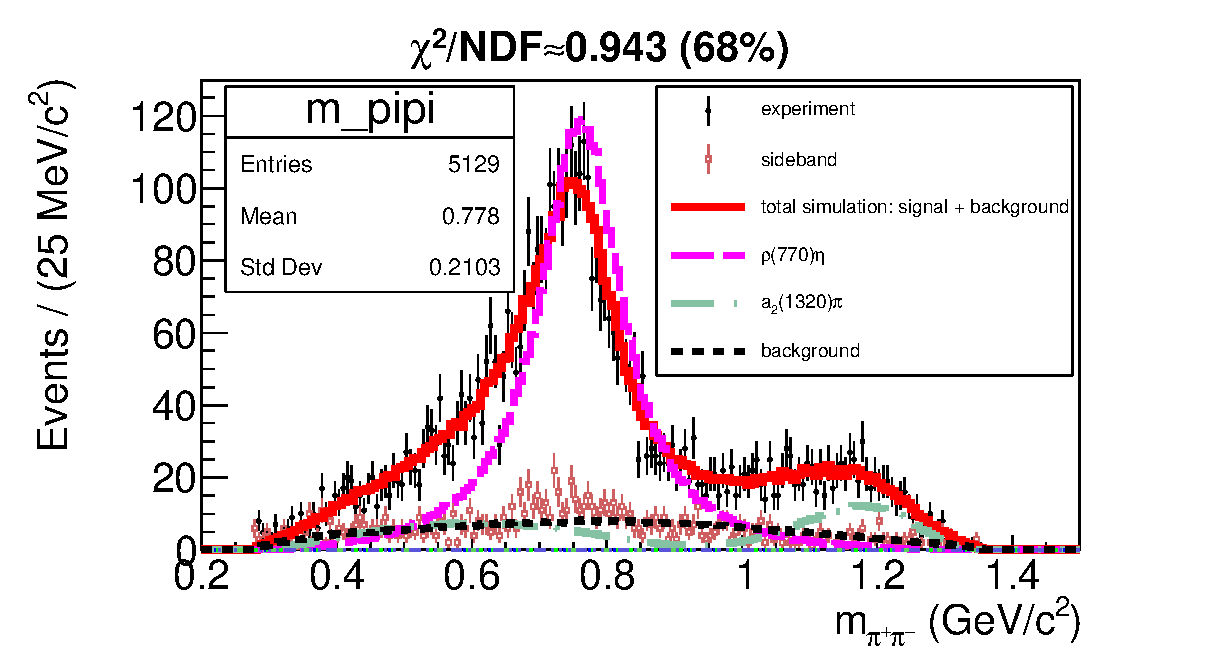
\includegraphics[width=\linewidth]{figures/m_pipi_g950.eps}
    \end{figure}
  \end{minipage}
  \begin{minipage}[t]{0.48\linewidth}
    \begin{figure}
      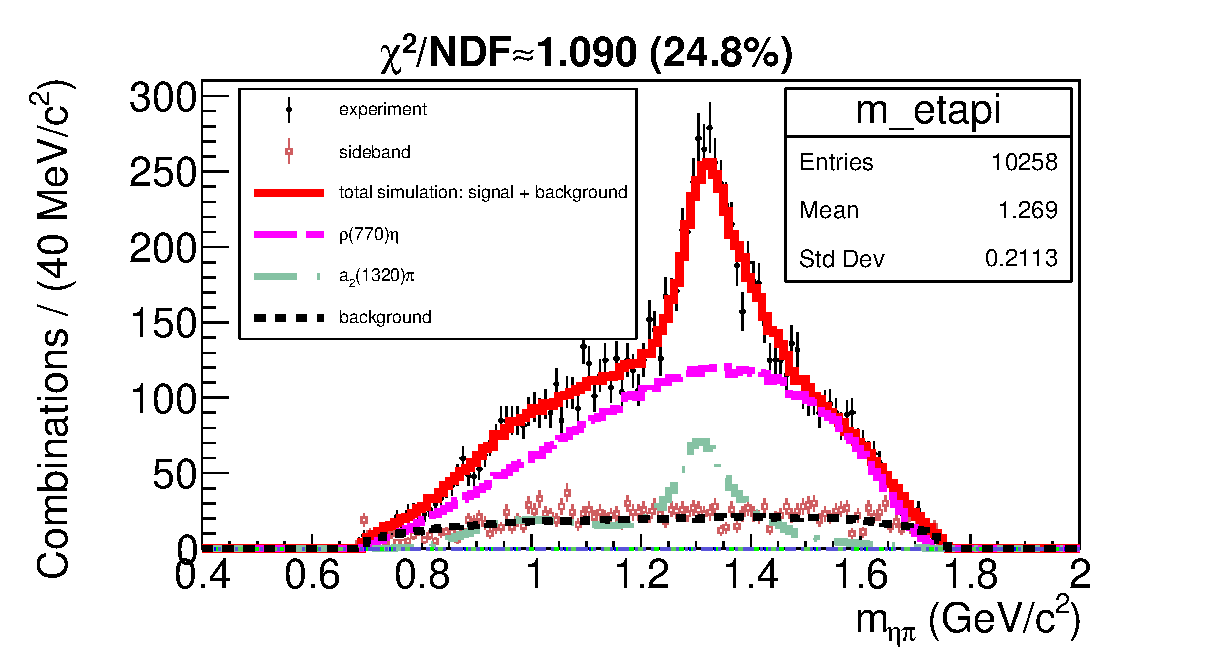
\includegraphics[width=\linewidth]{figures/m_etapi_g950.eps}
    \end{figure}
  \end{minipage}
  \begin{minipage}[t]{0.48\linewidth}
    \begin{figure}
      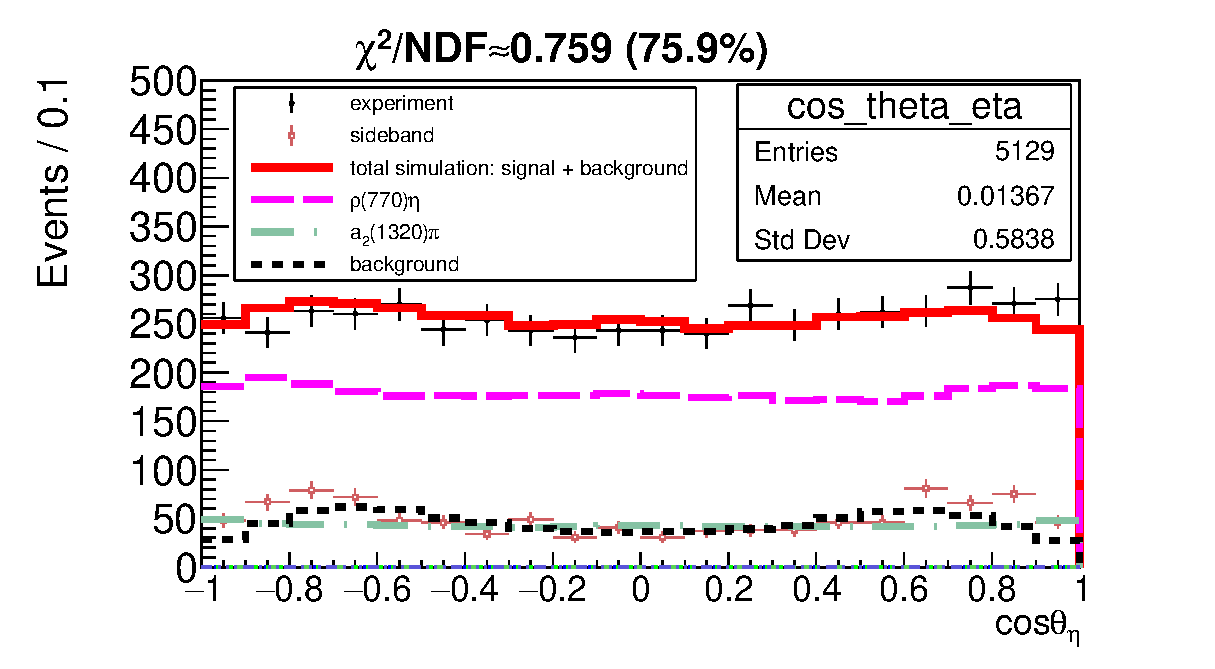
\includegraphics[width=\linewidth]{figures/cos_theta_eta_g950.eps}
    \end{figure}
  \end{minipage}
  \begin{minipage}[t]{0.48\linewidth}
    \begin{figure}
      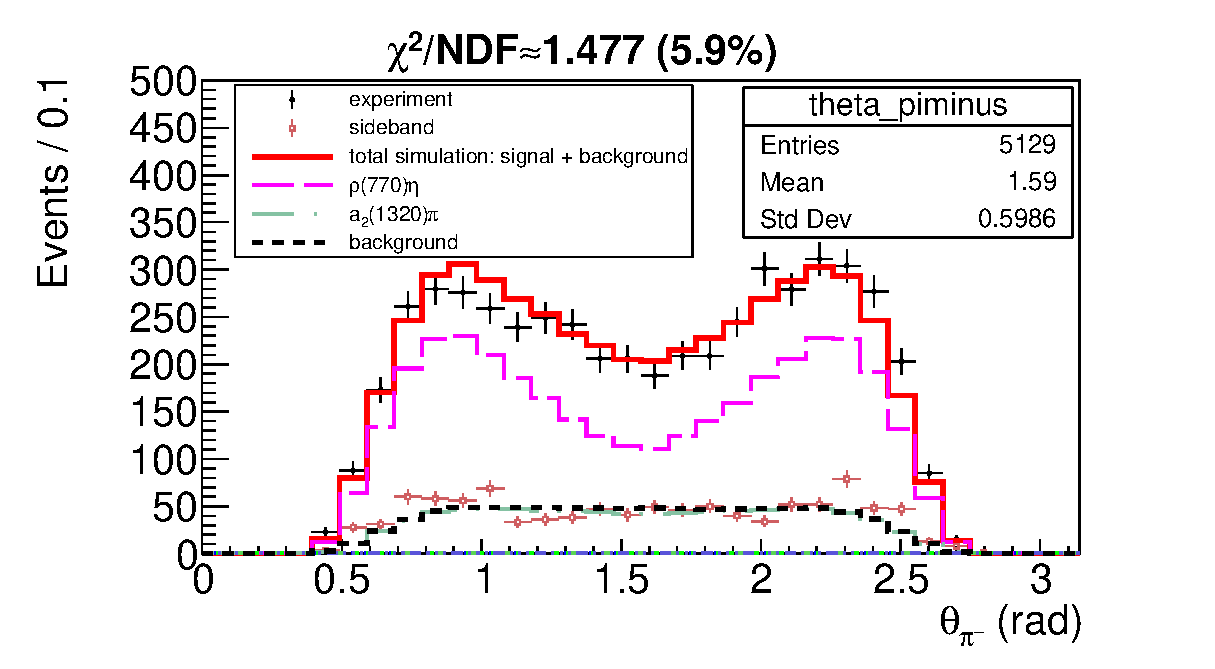
\includegraphics[width=\linewidth]{figures/theta_piminus_g950.eps}
    \end{figure}
  \end{minipage}
\end{frame}

\begin{frame}
  \frametitle{Сравнение спектров, $\sqrt{s}\approx{1.4}\text{ ГэВ}$}
  \begin{minipage}[t]{0.48\linewidth}
    \begin{figure}
      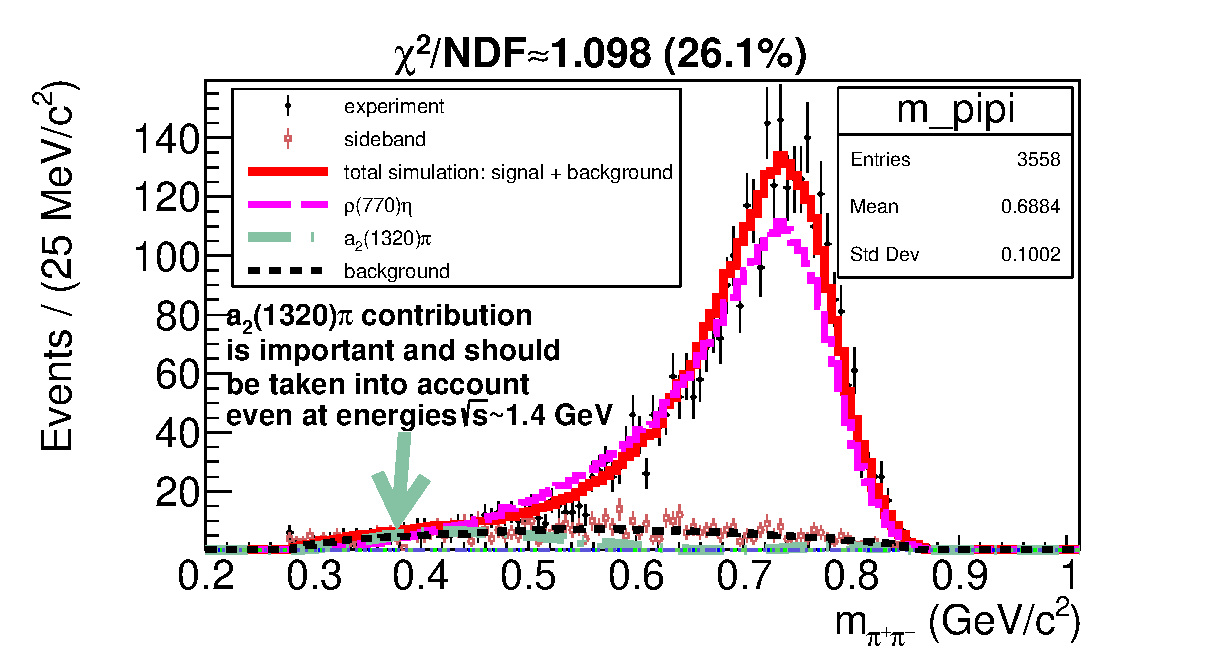
\includegraphics[width=\linewidth]{figures/m_pipi_g705.eps}
    \end{figure}
  \end{minipage}
  \begin{minipage}[t]{0.48\linewidth}
    \begin{figure}
      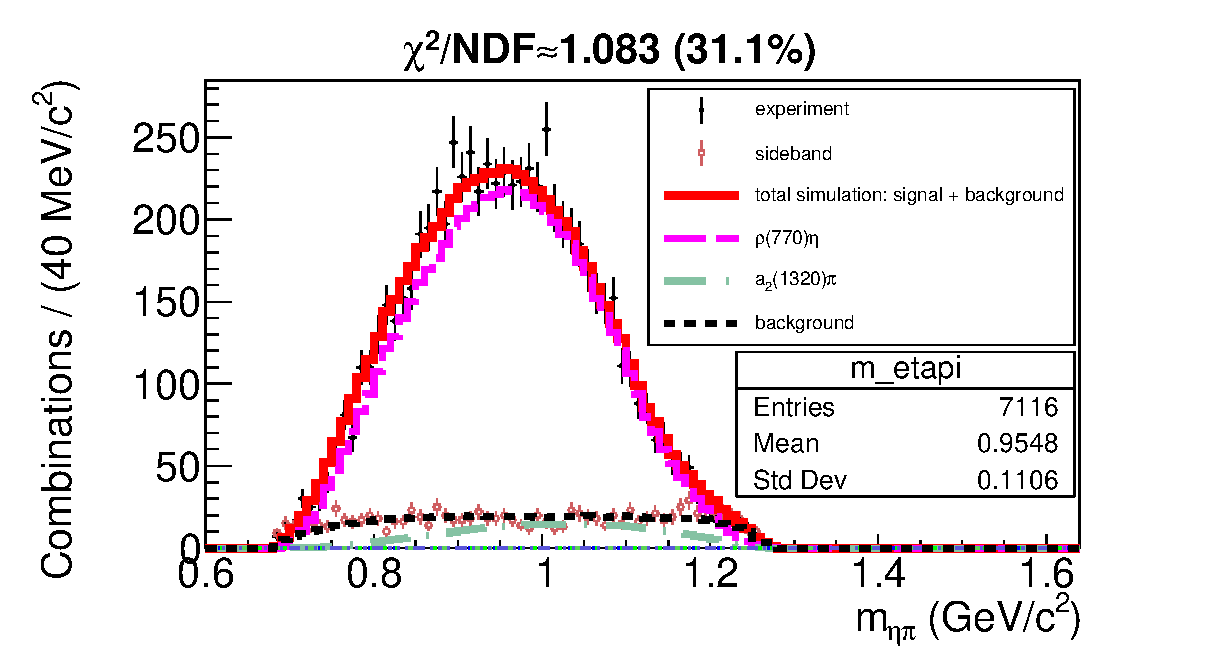
\includegraphics[width=\linewidth]{figures/m_etapi_g705.eps}
    \end{figure}
  \end{minipage}
  \begin{minipage}[t]{0.48\linewidth}
    \begin{figure}
      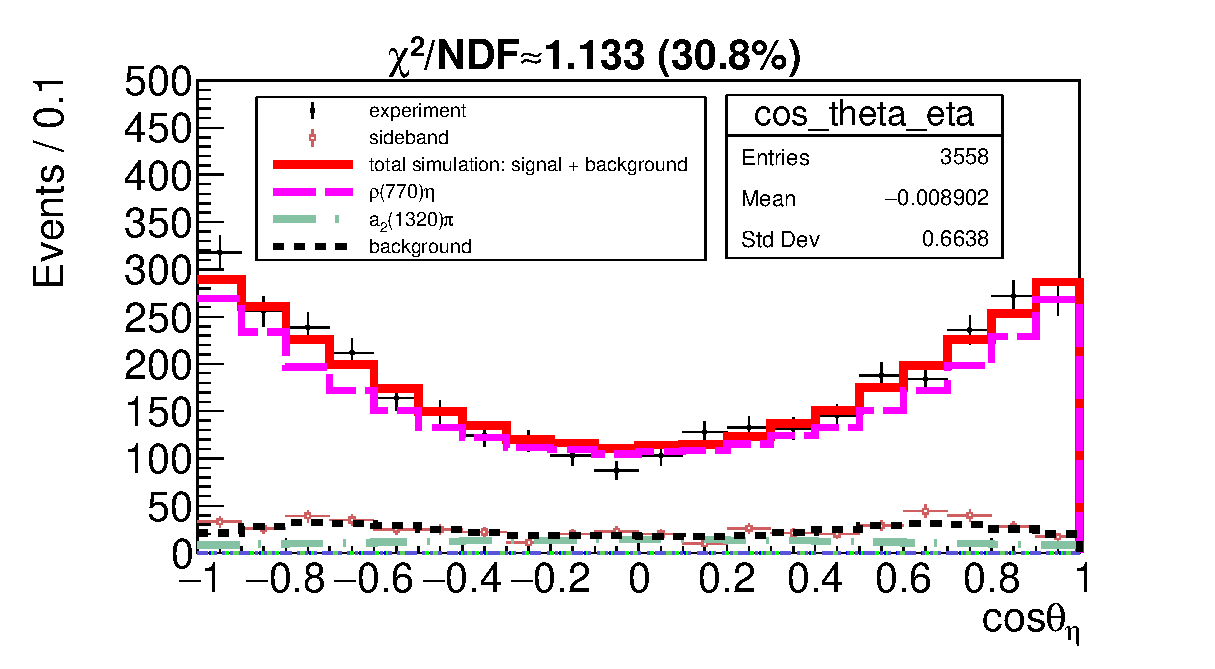
\includegraphics[width=\linewidth]{figures/cos_theta_eta_g705.eps}
    \end{figure}
  \end{minipage}
  \begin{minipage}[t]{0.48\linewidth}
    \begin{figure}
      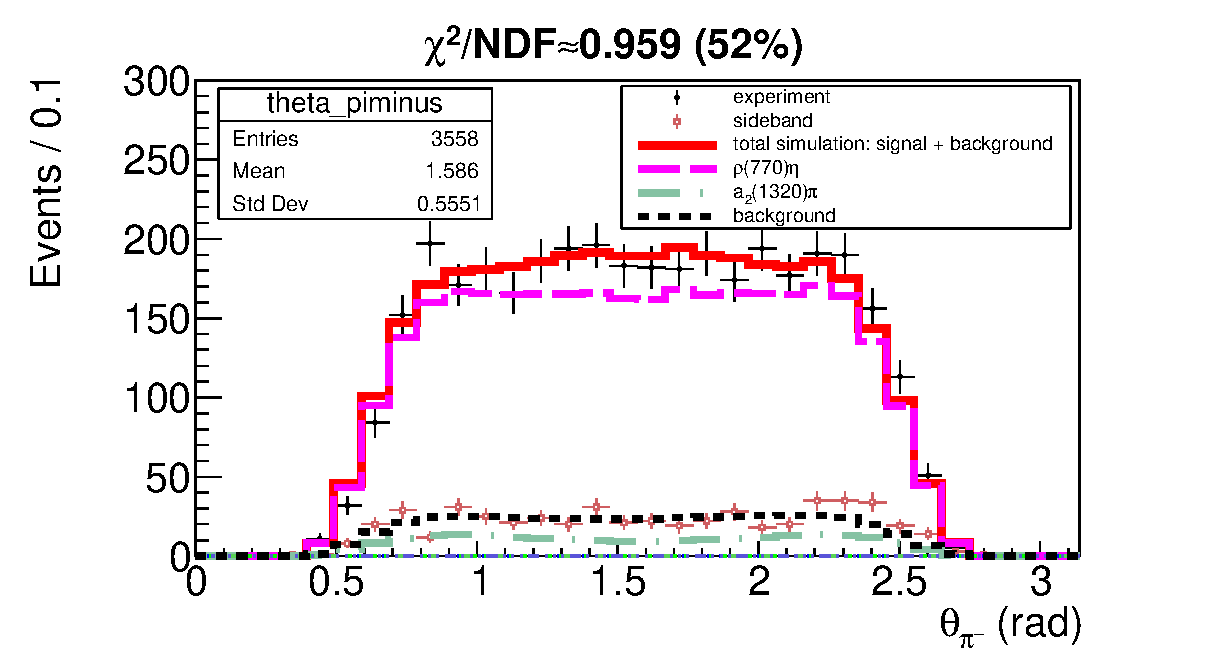
\includegraphics[width=\linewidth]{figures/theta_piminus_g705.eps}
    \end{figure}
  \end{minipage}
\end{frame}


\begin{frame}
  \frametitle{Сечение}
  \begin{minipage}[t]{0.48\linewidth}
    \begin{figure}
      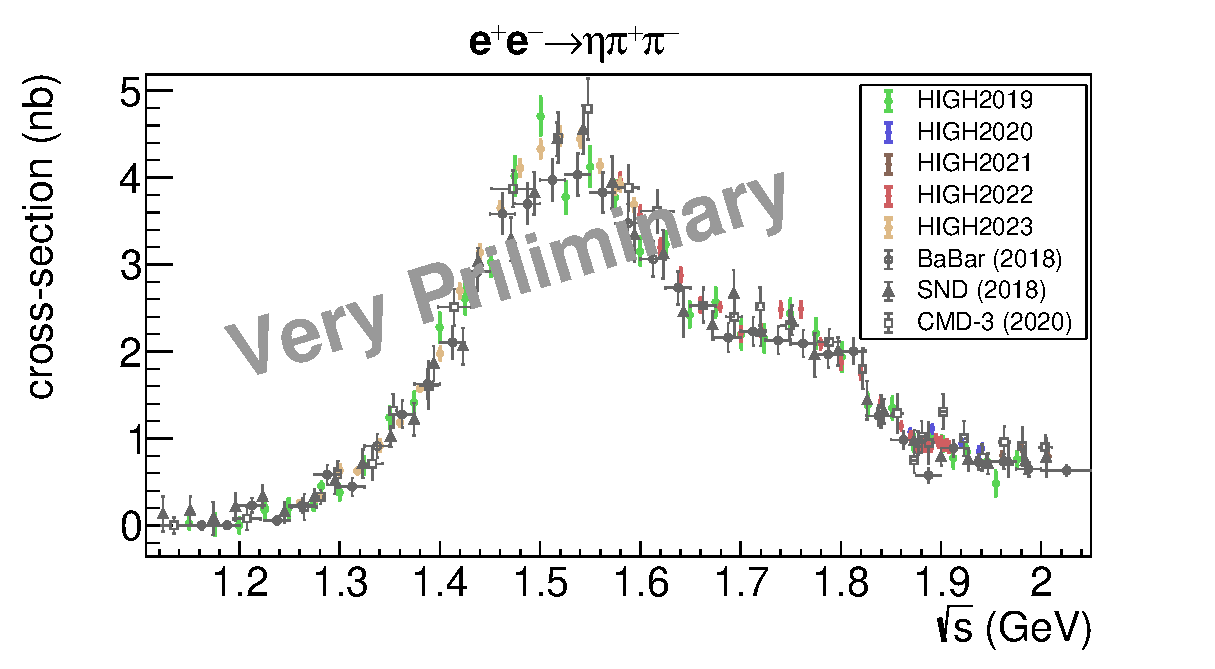
\includegraphics[width=\linewidth]{figures/bcs_etapipi.eps}
    \end{figure}
  \end{minipage}
  \begin{minipage}[t]{0.48\linewidth}
    \begin{figure}
      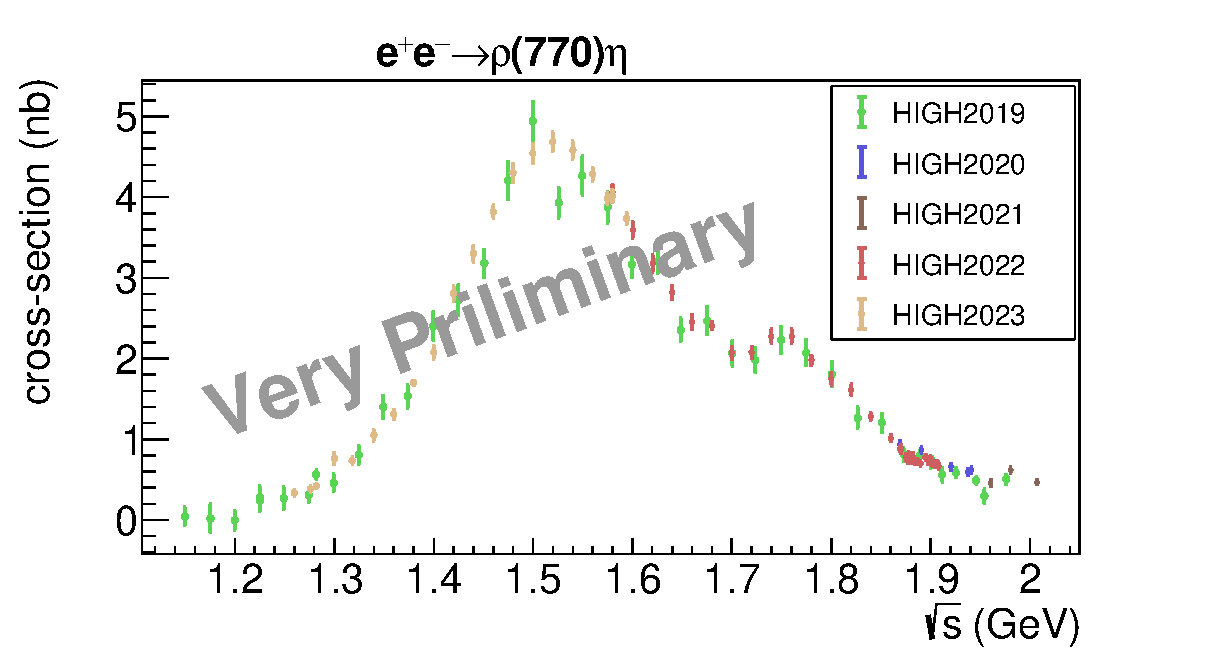
\includegraphics[width=\linewidth]{figures/bcs_partial_rhoeta.eps}
    \end{figure}
  \end{minipage}
  \begin{minipage}[t]{0.48\linewidth}
    \begin{figure}
      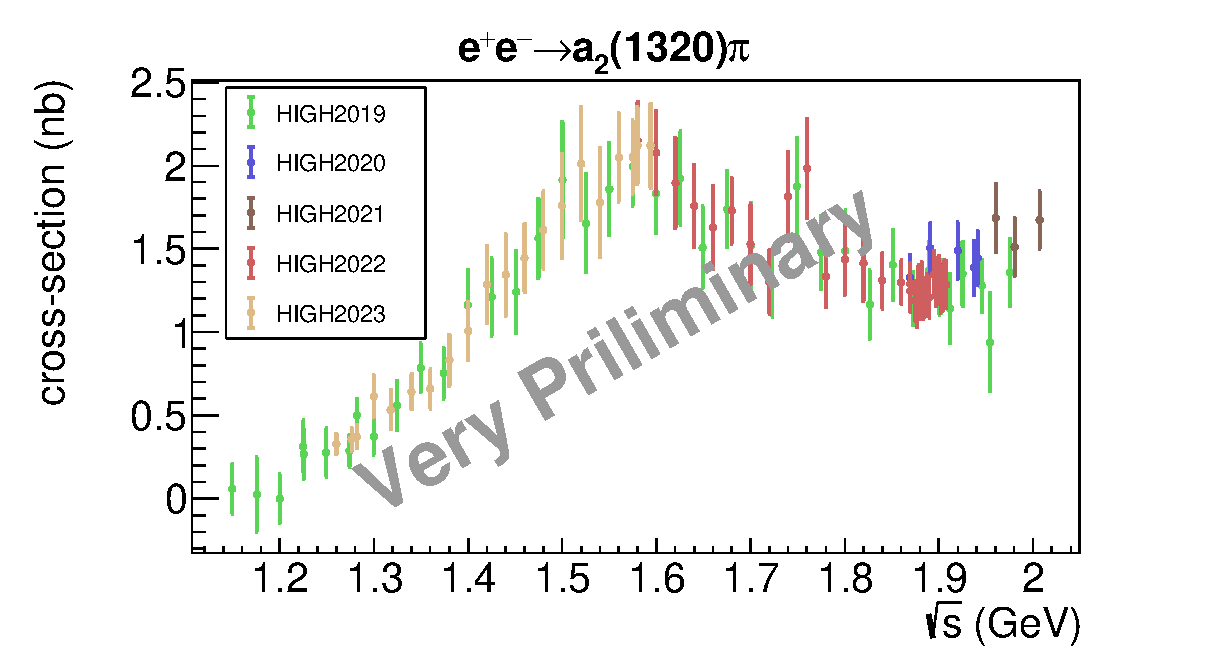
\includegraphics[width=\linewidth]{figures/bcs_partial_a2pi.eps}
    \end{figure}
  \end{minipage}
\end{frame}

\begin{frame}
  \frametitle{Уточнение модели фона}
\end{frame}


\end{document}
